\documentclass[tikz]{standalone}
\usepackage{graphicx}
\usepackage{tikz}
\usetikzlibrary{positioning}
\usetikzlibrary{calc}
\usetikzlibrary{backgrounds}
\usetikzlibrary{3d}
\usepackage{relsize}
\usetikzlibrary{decorations.pathreplacing}
\usetikzlibrary{arrows.meta}
\usepackage{amsmath}

\usepackage{fontspec}
\setmainfont[
 BoldFont={Varta-Bold.ttf}, 
 ]{Varta-Regular.ttf}
 
 
\newcommand{\drawcolor}{black}
\newcommand{\bgcolor}{white}
 

\definecolor{primary}{HTML}{FF9D00}
\definecolor{complement}{HTML}{0062FF}

\definecolor{ored}{HTML}{fa4405}
\definecolor{ogreen}{HTML}{06b050}
\definecolor{oblue}{HTML}{04b3ea}

\colorlet{main}{red!20!\bgcolor}

\colorlet{darkgr}{white!20!\drawcolor}

\colorlet{whitecomponentborder}{\drawcolor!70!\bgcolor}
\colorlet{whitecomponentfill}{\bgcolor!80!\drawcolor}

\colorlet{darkcomponentborder}{\bgcolor!70!\drawcolor}
\colorlet{darkcomponentfill}{\drawcolor!80!\bgcolor}

\colorlet{bluecomponentborder}{complement!80!\bgcolor}
\colorlet{bluecomponentfill}{complement!10!\bgcolor}

\colorlet{level}{complement!60!\bgcolor}
\colorlet{levelborder}{complement!50!\bgcolor}

\colorlet{environment}{ored!60!\bgcolor}
\colorlet{environmentborder}{ored!50!\drawcolor!30!\bgcolor}

\colorlet{componentborder}{main!200!\bgcolor}
\colorlet{componentfill}{main!40!\bgcolor}


\tikzstyle{redmodule}=[\drawcolor, solid, draw=componentborder, very thick, minimum width=25mm, fill=componentfill, text width=20mm]
\tikzstyle{bluemodule}=[\drawcolor, solid, draw=bluecomponentborder, very thick, minimum width=25mm, fill=bluecomponentfill, text width=20mm]
\tikzstyle{whitemodule}=[\drawcolor, solid, draw=whitecomponentborder, minimum width=10mm, fill=whitecomponentfill, text width=15mm]
\tikzstyle{darkmodule}=[\bgcolor, solid, draw=darkcomponentborder, minimum width=10mm, fill=darkcomponentfill, text width=15mm]


\begin{document}
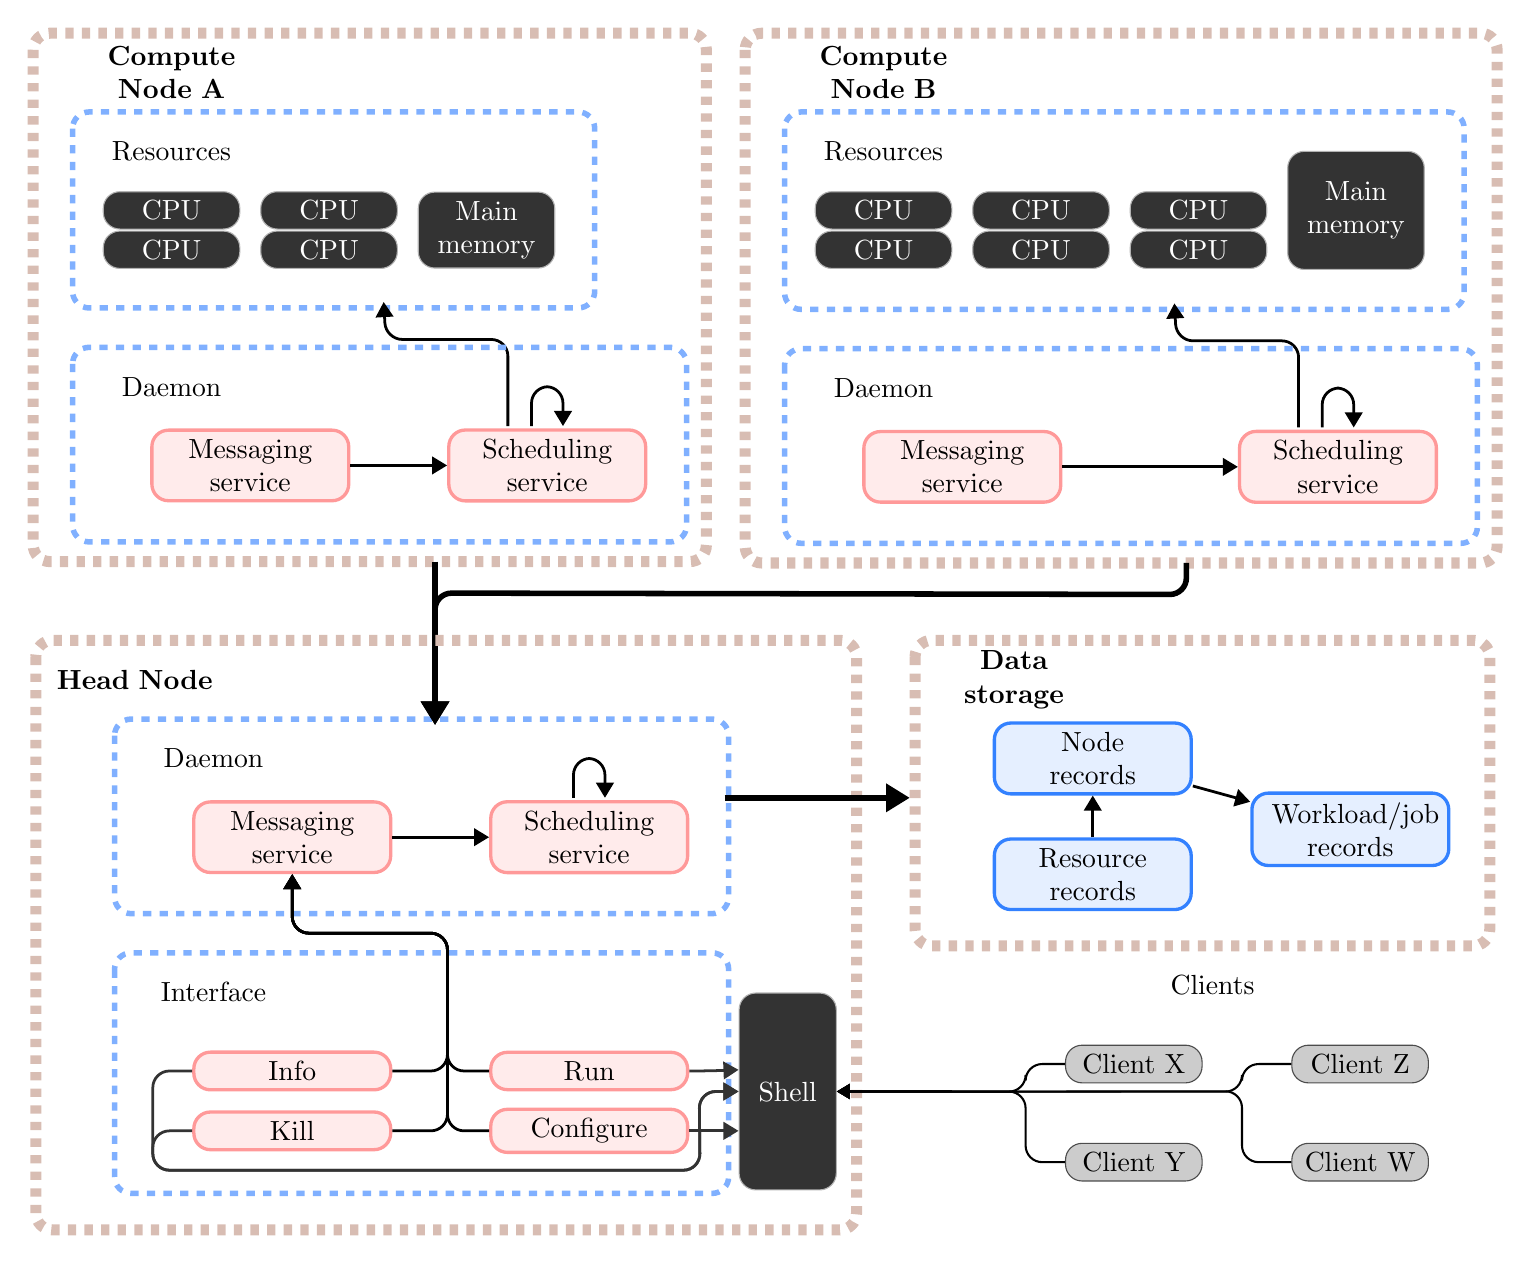
\begin{tikzpicture}[rounded corners=6, align=center]
    \begin{scope}[local bounding box=model]
        %%%%%%%%%%%%%%%%%%%%%%%%%%%%%%%%%%%%%%%%%%%%%%%%%%
        % Compute node A
        %%%%%%%%%%%%%%%%%%%%%%%%%%%%%%%%%%%%%%%%%%%%%%%%%%
        \node[\drawcolor, solid, text width=30mm, minimum width=35mm] at (-2, 2) (computeAnodetitle) {\textbf{Compute Node A}};

        %%%%%%%%%%%%%%%%%%%%%%%%%%%%%%%
        % RESOURCES
        %%%%%%%%%%%%%%%%%%%%%%%%%%%%%%

        \node[\drawcolor, solid, text width=20mm, minimum width=25mm] at ($(computeAnodetitle) + (0.0, -1.0)$)
            (computeAResourceTitle) {Resources};

        \node[darkmodule] at ($(computeAResourceTitle) + (0, -0.75)$) (computeACPU0) {CPU};
        \node[darkmodule] at ($(computeACPU0) + (2.0, 0.0)$) (computeACPU1) {CPU};
        \node[darkmodule] at ($(computeACPU0) + (0.0, -0.5)$) (computeACPU2) {CPU};
        \node[darkmodule] at ($(computeACPU1) + (0.0, -0.5)$) (computeACPU3) {CPU};
        \node[darkmodule] at ($(computeACPU0) + (4.0, -0.25)$) (computeARAM) {Main memory};

        % Resource border
        \draw[dashed, draw=levelborder, line width=2pt] ($(computeAResourceTitle.west) + (-0.0, 0.5)$) rectangle
            ($(computeARAM.south east) + (0.5, -0.5)$) node (computeAResourcesCorner) {};

        % Meta
        \path let \p1 = (computeAResourceTitle), \p2 = (computeAResourcesCorner) in node (computeAResources) at ($(\x1, \y2) + (-1.0, 0)$) {};
        \path let \p1 = (computeAResourceTitle), \p2 = (computeAResourcesCorner) in node (computeAResourcesMiddle) at ($(\x1 / 2, \y2) + (\x2 / 2, 0.2)$) {};

        %%%%%%%%%%%%%%%%%%%%%%%%%%%%%%%
        % DAEMON
        %%%%%%%%%%%%%%%%%%%%%%%%%%%%%%

        \node[\drawcolor, solid, text width=20mm, minimum width=25mm] at ($(computeAResources) + (1.0, -1.0)$) (computeAdaemontitle) {Daemon};

        \node[redmodule] at ($(computeAdaemontitle) + (1, -1)$) (computeAmessaging) {Messaging service};

        \node[redmodule] at ($(computeAmessaging.east) + (2.5, 0.0)$) (computeAscheduling) {Scheduling service};

        % Arrows
        \draw[\drawcolor, -{Triangle}, line width=1pt] (computeAmessaging) to (computeAscheduling);
        \draw[\drawcolor, -{Triangle}, line width=1pt] ($(computeAscheduling) + (-0.2, 0.5)$) to ($(computeAscheduling) + (-0.2, 1.0)$) to ($(computeAscheduling) + (0.2, 1.0)$) to ($(computeAscheduling) + (0.2, 0.5)$);
        \draw[\drawcolor, -{Triangle}, line width=1pt] ($(computeAscheduling) + (-0.5, 0.5)$) to 
            ($(computeAscheduling) + (-0.5, 1.6)$) to
            ($(computeAscheduling) + (-2.05, 1.6)$) to
            (computeAResourcesMiddle);

        % Daemon border
        \draw[dashed, draw=levelborder, line width=2pt] ($(computeAdaemontitle.west) + (-0.0, 0.5)$) rectangle ($(computeAscheduling.south east) + (0.5, -0.5)$) node (computeAdaemon) {};

        %%% Compute node border
        \draw[dashed, draw=environmentborder, line width=4pt] ($(computeAnodetitle.west) + (-0.0, 0.5)$) rectangle
            ($(computeAscheduling.south east) + (0.75, -0.75)$) node (computeAcorner) {};

        % Meta
        \path let \p1 = (computeAcorner), \p2 = (computeAnodetitle) in node (computeATopRight) at ($(\x1, \y2) + (0, 0)$) {};
        \path let \p1 = (computeAcorner), \p2 = (computeAnodetitle) in node (computeAnode) at ($(\x1 / 2, \y1 / 2) + (\x2 / 2, \y2 / 2)$) {};
        \path let \p1 = (computeAcorner), \p2 = (computeAnode) in node (computeAbottom) at ($(\x2, \y1)$) {};
        \path let \p1 = (computeAcorner), \p2 = (computeAnodetitle.west) in node (computeAbottomleft) at ($(\x2, \y1) + (1.29, 0.0)$) {};

        %%%%%%%%%%%%%%%%%%%%%%%%%%%%%%%%%%%%%%%%%%%%%%%%%%
        % Compute node B
        %%%%%%%%%%%%%%%%%%%%%%%%%%%%%%%%%%%%%%%%%%%%%%%%%%
        \node[\drawcolor, solid, text width=30mm, minimum width=35mm] at ($(computeATopRight) + (2.25, 0)$) (computeBnodetitle)
            {\textbf{Compute Node B}};

        %%%%%%%%%%%%%%%%%%%%%%%%%%%%%%%
        % RESOURCES
        %%%%%%%%%%%%%%%%%%%%%%%%%%%%%%

        \node[\drawcolor, solid, text width=20mm, minimum width=25mm] at ($(computeBnodetitle) + (0.0, -1.0)$)
            (computeBResourceTitle) {Resources};

        \node[darkmodule] at ($(computeBResourceTitle) + (0, -0.75)$) (computeBCPU0) {CPU};
        \node[darkmodule] at ($(computeBCPU0) + (2.0, 0.0)$) (computeBCPU1) {CPU};
        \node[darkmodule] at ($(computeBCPU0) + (0.0, -0.5)$) (computeBCPU2) {CPU};
        \node[darkmodule] at ($(computeBCPU1) + (0.0, -0.5)$) (computeBCPU3) {CPU};
        \node[darkmodule] at ($(computeBCPU1) + (2.0, 0.0)$) (computeBCPU4) {CPU};
        \node[darkmodule] at ($(computeBCPU4) + (0.0, -0.5)$) (computeBCPU5) {CPU};
        \node[darkmodule, minimum height=15mm] at ($(computeBCPU4) + (2.0, 0.0)$) (computeBRAM) {Main memory};

        % Resource border
        \draw[dashed, draw=levelborder, line width=2pt] ($(computeBResourceTitle.west) + (-0.0, 0.5)$) rectangle
            ($(computeBRAM.south east) + (0.5, -0.5)$) node (computeBResourcesCorner) {};

        % Meta
        \path let \p1 = (computeBResourceTitle), \p2 = (computeBResourcesCorner) in node (computeBResources) at ($(\x1, \y2) + (-1.0, 0)$) {};
        \path let \p1 = (computeBResourceTitle), \p2 = (computeBResourcesCorner) in node (computeBResourcesMiddle) at ($(\x1 / 2, \y2) + (\x2 / 2, 0.2)$) {};

        %%%%%%%%%%%%%%%%%%%%%%%%%%%%%%%
        % DAEMON
        %%%%%%%%%%%%%%%%%%%%%%%%%%%%%%

        \node[\drawcolor, solid, text width=20mm, minimum width=25mm] at ($(computeBResources) + (1.0, -1.0)$) (computeBdaemontitle) {Daemon};

        \node[redmodule] at ($(computeBdaemontitle) + (1, -1)$) (computeBmessaging) {Messaging service};

        \node[redmodule] at ($(computeBmessaging.east) + (3.5, 0.0)$) (computeBscheduling) {Scheduling service};

        % Arrows
        \draw[\drawcolor, -{Triangle}, line width=1pt] (computeBmessaging) to (computeBscheduling);
        \draw[\drawcolor, -{Triangle}, line width=1pt] ($(computeBscheduling) + (-0.2, 0.5)$) to ($(computeBscheduling) + (-0.2, 1.0)$) to ($(computeBscheduling) + (0.2, 1.0)$) to ($(computeBscheduling) + (0.2, 0.5)$);
        \draw[\drawcolor, -{Triangle}, line width=1pt] ($(computeBscheduling) + (-0.5, 0.5)$) to 
            ($(computeBscheduling) + (-0.5, 1.6)$) to
            ($(computeBscheduling) + (-2.05, 1.6)$) to
            (computeBResourcesMiddle);

        % Daemon border
        \draw[dashed, draw=levelborder, line width=2pt] ($(computeBdaemontitle.west) + (-0.0, 0.5)$) rectangle ($(computeBscheduling.south east) + (0.5, -0.5)$) node (computeBdaemon) {};

        %%% Compute node border
        \draw[dashed, draw=environmentborder, line width=4pt] ($(computeBnodetitle.west) + (-0.0, 0.5)$) rectangle
            ($(computeBscheduling.south east) + (0.75, -0.75)$) node (computeBcorner) {};

        % Meta
        \path let \p1 = (computeBcorner), \p2 = (computeBnodetitle) in node (computeBnode) at ($(\x1 / 2, \y1 / 2) + (\x2 / 2, \y2 / 2)$) {};
        \path let \p1 = (computeBcorner), \p2 = (computeBnode) in node (computeBbottom) at ($(\x2, \y1)$) {};
        \path let \p1 = (computeBcorner), \p2 = (computeBnodetitle.west) in node (computeBbottomleft) at ($(\x2, \y1) + (1.29, 0.0)$) {};


        %%%%%%%%%%%%%%%%%%%%%%%%%%%%%%%%%%%%%%%%%%%%%%%%%%
        % Head node
        %%%%%%%%%%%%%%%%%%%%%%%%%%%%%%%%%%%%%%%%%%%%%%%%%%
        \node[\drawcolor, solid, text width=20mm, minimum width=25mm] at ($(computeAbottomleft) + (0.0, -1.5)$) (headnodetitle)
            {\textbf{Head Node}};

        %%%%%%%%%%%%%%%%%%%%%%%%%%%%%%%
        % DAEMON
        %%%%%%%%%%%%%%%%%%%%%%%%%%%%%%

        \node[\drawcolor, solid, text width=20mm, minimum width=25mm] at ($(headnodetitle) + (1.0, -1.0)$) (headdaemontitle) {Daemon};

        \node[redmodule] at ($(headdaemontitle) + (1, -1)$) (headmessaging) {Messaging service};

        \node[redmodule] at ($(headmessaging.east) + (2.5, 0.0)$) (headscheduling) {Scheduling service};

        % Arrows
        \draw[\drawcolor, -{Triangle}, line width=1pt] (headmessaging) to (headscheduling);
        \draw[\drawcolor, -{Triangle}, line width=1pt] ($(headscheduling) + (-0.2, 0.5)$) to ($(headscheduling) + (-0.2, 1.0)$) to ($(headscheduling) + (0.2, 1.0)$) to ($(headscheduling) + (0.2, 0.5)$);

        % Daemon border
        \draw[dashed, draw=levelborder, line width=2pt] ($(headdaemontitle.west) + (-0.0, 0.5)$) rectangle ($(headscheduling.south east) + (0.5, -0.5)$) node (headdaemon) {};
    
        % Compute A --> Head
        \path let \p1 = (computeAbottom), \p2 = (headnodetitle) in node (headLinkA) at ($(\x1, \y2) + (-0.05, -0.7)$) {};
        \draw[\drawcolor, -{Triangle}, line width=2pt] ($(computeAbottom) + (-0.05, 0.0)$) to (headLinkA);
    
        % Compute B --> Head
        \draw[\drawcolor, -{Triangle}, line width=2pt] ($(computeBbottom) + (-0.05, 0.0)$) to 
            ($(computeBbottom) + (-0.05, -0.4)$) to 
            ($(computeAbottom) + (-0.05, -0.4)$) to 
            (headLinkA);

        %%%%%%%%%%%%%%%%%%%%%%%%%%%%%%%
        % INTERFACE
        %%%%%%%%%%%%%%%%%%%%%%%%%%%%%%
        \path let \p1 = (headdaemontitle), \p2 = (headmessaging.south) in node (intstart) at ($(\x1, \y2) + (0, -1.5)$) {};

        \node[\drawcolor, solid, text width=20mm, minimum width=25mm] at (intstart) (interfacetitle) {Interface};

        \node[redmodule] at ($(interfacetitle) + (1, -1)$) (infomodule) {Info};

        \node[redmodule] at ($(infomodule.east) + (2.5, 0.0)$) (runmodule) {Run};

        \node[redmodule] at ($(infomodule.south) + (0.0, -0.5)$) (killmodule) {Kill};

        \node[redmodule] at ($(killmodule.east) + (2.5, 0.0)$) (configuremodule) {Configure};

        \node[darkmodule, minimum height=25mm, minimum width=1mm, text width=10mm] at ($(configuremodule.east) + (1.25, 0.5)$) (headshell) {Shell};

        % Arrows
        \draw[\drawcolor, -{Triangle}, line width=1pt] ($(infomodule.east) + (-0.0, 0.0)$) to ($(infomodule.east) + (0.7, 0.0)$) to
            ($(infomodule.east) + (0.7, 1.75)$) to ($(headmessaging.south) + (0.0, -0.75)$) to ($(headmessaging.south) + (0.0, 0.0)$);
        \draw[\drawcolor, -{Triangle}, line width=1pt] ($(runmodule.west) + (-0.0, 0.0)$) to ($(infomodule.east) + (0.7, 0.0)$) to
            ($(infomodule.east) + (0.7, 1.75)$) to ($(headmessaging.south) + (0.0, -0.75)$) to ($(headmessaging.south) + (0.0, 0.0)$);
        \draw[\drawcolor, -{Triangle}, line width=1pt] ($(killmodule.east) + (-0.0, 0.0)$) to ($(killmodule.east) + (0.7, 0.0)$) to ($(infomodule.east) + (0.7, 0.0)$) to
            ($(infomodule.east) + (0.7, 1.75)$) to ($(headmessaging.south) + (0.0, -0.75)$) to ($(headmessaging.south) + (0.0, 0.0)$);
        \draw[\drawcolor, -{Triangle}, line width=1pt] ($(configuremodule.west) + (-0.0, 0.0)$) to ($(killmodule.east) + (0.7, 0.0)$) to ($(infomodule.east) + (0.7, 0.0)$) to
            ($(infomodule.east) + (0.7, 1.75)$) to ($(headmessaging.south) + (0.0, -0.75)$) to ($(headmessaging.south) + (0.0, 0.0)$);

        % Interface border
        \draw[dashed, draw=levelborder, line width=2pt] ($(interfacetitle.west) + (-0.0, 0.5)$) rectangle ($(configuremodule.south east) + (0.5, -0.5)$);

        % Shell arrows
        \draw[darkgr, -{Triangle}, line width=1pt] (runmodule.east) to ($(runmodule.east) + (0.25, 0.0)$) to 
            ($(headshell.west) + (0.0, 0.275)$);
        \draw[darkgr, -{Triangle}, line width=1pt] (configuremodule.east) to ($(configuremodule.east) + (0.25, 0.0)$) to 
            ($(headshell.west) + (0.0, -0.5)$);
        \draw[darkgr, -{Triangle}, line width=1pt] (killmodule.west) to ($(killmodule.west) + (-0.5, 0.0)$) to
            ($(killmodule.west) + (-0.5, -0.5)$) to ($(killmodule.west) + (6.45, -0.5)$) to
            ($(headshell.west) + (-0.5, 0.0)$) to (headshell.west);
        \draw[darkgr, -{Triangle}, line width=1pt] (infomodule.west) to ($(infomodule.west) + (-0.5, 0.0)$) to
            ($(killmodule.west) + (-0.5, 0.0)$) to
            ($(killmodule.west) + (-0.5, -0.5)$) to ($(killmodule.west) + (6.45, -0.5)$) to
            ($(headshell.west) + (-0.5, 0.0)$) to (headshell.west);

        %%% Head node border
        \draw[dashed, draw=environmentborder, line width=4pt] ($(headnodetitle.west) + (-0.0, 0.5)$) rectangle
            ($(headshell.south east) + (0.25, -0.5)$) node (headcorner) {};

        % Meta
        \path let \p1 = (headcorner), \p2 = (headnodetitle) in node (headnode) at ($(\x1 / 2, \y1 / 2) + (\x2 / 2, \y2 / 2)$) {};
        \path let \p1 = (headcorner), \p2 = (headnode) in node (headbottom) at ($(\x2, \y1)$) {};
        \path let \p1 = (headcorner), \p2 = (headnode) in node (headright) at ($(\x1, \y2)$) {};
        
        %%%%%%%%%%%%%%%%%%%%%%%%%%%%%%%%%%%%%%%%%%%%%%%%%%
        % Database
        %%%%%%%%%%%%%%%%%%%%%%%%%%%%%%%%%%%%%%%%%%%%%%%%%%
        \path let \p1 = (headright), \p2 = (headnodetitle) in node (dbstart) at ($(\x1, \y2) + (2, -0.0)$) {};
        \path let \p1 = (headdaemon), \p2 = (headnodetitle) in node (dblink) at ($(\x1, \y2) + (0.0, -1.5)$) {};

        \node[\drawcolor, solid, text width=20mm, minimum width=25mm] at (dbstart) (databasetitle) {\textbf{Data storage}};

        \node[bluemodule] at ($(databasetitle) + (1, -1)$) (nodetable) {Node records};

        \node[bluemodule] at ($(nodetable.south) + (0.0, -1.0)$) (resourcetable) {Resource records};

        \node[bluemodule] at ($(nodetable.east) + (2.0, -0.9)$) (jobtable) {Workload/job records};

        % Database border
        \draw[dashed, draw=environmentborder, line width=4pt] ($(databasetitle.west) + (-0.0, 0.5)$) rectangle ($(jobtable.south east) + (0.5, -1.0)$) node (databasecorner) {};

        \draw[\drawcolor, -{Triangle}, line width=1pt] (resourcetable) to (nodetable);
        \draw[\drawcolor, -{Triangle}, line width=1pt] (nodetable) to (jobtable);
    
        % Head --> database
        \draw[\drawcolor, -{Triangle}, line width=2pt] ($(dblink) + (-0.05, 0.0)$) to ($(dblink) + (2.3, 0)$);

        % Meta
        \path let \p1 = (databasecorner), \p2 = (databasetitle) in node (database) at ($(\x1 / 2, \y1 / 2) + (\x2 / 2, \y2 / 2)$) {};
        \path let \p1 = (databasecorner), \p2 = (database) in node (databasebottom) at ($(\x2, \y1)$) {};
        
        %%%%%%%%%%%%%%%%%%%%%%%%%%%%%%%%%%%%%%%%%%%%%%%%%%
        % Client
        %%%%%%%%%%%%%%%%%%%%%%%%%%%%%%%%%%%%%%%%%%%%%%%%%%
        \path let \p1 = (databasebottom) in node (clientstart) at ($(\x1, \y1) + (-0.5, -0.5)$) {};

        \node[\drawcolor, solid, text width=20mm, minimum width=25mm] at (clientstart) (clienttitle) {Clients};

        \node[whitemodule] at ($(clienttitle) + (-1.0, -1.0)$) (client1) {Client X};

        \node[whitemodule] at ($(client1.south) + (0.0, -1.0)$) (client2) {Client Y};

        \node[whitemodule] at ($(client1.east) + (2.0, -0.0)$) (client3) {Client Z};

        \node[whitemodule] at ($(client3.south) + (0.0, -1.0)$) (client4) {Client W};

        % Arrows
        \draw[\drawcolor, -{Triangle}, line width=0.75pt] (client1.west) to ($(client1.west) + (-0.5, 0.0)$) to
            ($(client1.west) + (-0.5, -0.35)$) to ($(headshell.east) + (0.5, 0.0)$) to (headshell.east);
        \draw[\drawcolor, -{Triangle}, line width=0.75pt] (client2.west) to ($(client2.west) + (-0.5, 0.0)$) to
            ($(client1.west) + (-0.5, -0.35)$) to ($(headshell.east) + (0.5, 0.0)$) to (headshell.east);
        \draw[\drawcolor, -{Triangle}, line width=0.75pt] (client3.west) to ($(client1.east) + (0.5, 0.0)$) to
            ($(client1.east) + (0.5, -0.35)$) to
            ($(client1.west) + (-0.5, -0.35)$) to ($(headshell.east) + (0.5, 0.0)$) to (headshell.east);
        \draw[\drawcolor, -{Triangle}, line width=0.75pt] (client4.west) to ($(client2.east) + (0.5, 0.0)$) to
            ($(client2.east) + (0.5, 0.9)$) to
            ($(client1.west) + (-0.5, -0.35)$) to ($(headshell.east) + (0.5, 0.0)$) to (headshell.east);

    \end{scope}

\end{tikzpicture}
\end{document}
